\graphicspath{{images/}} %Indicação da pasta de imagens

%C para centralizar verticalmente o que for escrito. Transfade é o efeito por 0.3 segundos
%Tipos de efeito do Beamer: Mais informações em
%http://tug.ctan.org/macros/latex/contrib/beamer/doc/beameruserguide.pdf página 144

%\transblindshorizontal Mostra o slide como se cortinas horizontais fossem puxadas

% \transblindsvertical Mostra o slide como se cortinas verticais fossem puxadas

%\transboxin Mostra o slide movendo para o centro dos quatro cantos

%\transboxout Contrario do boxin

%\transdissolve Dissolve lentamente o que foi mostrado antes

%\transglitter Glitter se move numa direção específica

%\transsplitverticalin Show the slide by sweeping two vertical lines from the sides inward.

%\transsplitverticalout Show the slide by sweeping two vertical lines from the center outward.

%\transsplithorizontalin Show the slide by sweeping two horizontal lines from the sides inward.

%\transsplithorizontalout Show the slide by sweeping two horizontal lines from the center outward.

%\transwipe Sweeps single line in specified direction

%\transduration{2} Show slide specified number of seconds

%\transpush Show the slide by pushing what was shown before off the screen using the new content.

%\transreplace Replace the previous slide directly (default behaviour).

%\transfade
%\transpush
%\transuncover

%\transcover Show the slide by covering the content that was shown before



%%%%%%%%%%%%%%%%%% SLIDE 1 %%%%%%%%%%%%%%%%%%%%
\begin{frame}[c]\transfade<1>[duration=0.3]
\section{Introdução}
\frametitle{Introdução} 
%\framesubtitle{Subtítulo do Slide}
\begin{itemize}
    \justifying
    \item P-valor ou valor p é outro meio de relatar os resultados de um teste de hipótese.
    \item Um valor p relata os resultados de um teste em uma escala mais contínua, em vez de apenas ``aceitar $H_0$'' ou ``rejeitar $H_0$''.
\end{itemize}
\end{frame}

%%%%%%%%%%%%%%%%%% SLIDE 2 %%%%%%%%%%%%%%%%%%%%
\begin{frame}[c]\transfade<1>[duration=0.3]
\section{P-valor}
\frametitle{P-valor} 
\framesubtitle{Definição}
\begin{itemize}
    \justifying
    \item \textbf{Definição}: Um \textit{valor p p}(\textbf{X}) é uma estatística de teste que satisfaz $0 \leq p(\textbf{x}) \leq 1$ para cada ponto amostral \textbf{x}. Pequenos valores de \textit{p}(\textbf{X}) fornecem evidências de que $H_{1}$ é verdadeira. Um valor p é \textit{válido} se, para cada $\theta \in \Theta_{0}$ e cada $0 \leq \alpha \leq 1$,
\end{itemize}

\begin{equation}
     P_{ \theta } (p(\textbf{X})  \leq  \alpha ) \leq  \alpha.
\end{equation}
\end{frame}

%%%%%%%%%%%%%%%%%% SLIDE 3 %%%%%%%%%%%%%%%%%%%%
\begin{frame}[c]\transfade<1>[duration=0.3] 
\frametitle{P-valor} 
\framesubtitle{Definição}
\begin{equation}
     P_{ \theta } (p(\textbf{X})  \leq  \alpha ) \leq  \alpha.
\end{equation}
Onde,
\begin{itemize}
    \item $P_{ \theta }$ declara a probabilidade de ocorrência de eventos extremos (rejeitar a hipótese nula sabendo que é verdadeira);
    \item $p(\textbf{X})$ é uma estatística de teste sob a população em estudo e
    \item $\alpha$ denota o nível de significância estipulado.
\end{itemize}
\end{frame}

%%%%%%%%%%%%%%%%%% SLIDE 4 %%%%%%%%%%%%%%%%%%%%
\begin{frame}[c]\transfade<1>[duration=0.3] 
\frametitle{P-valor} 
\framesubtitle{Teorema}
\begin{itemize}
    \justifying
    \item O meio mais comum para definir um valor p válido é dado por:
    \item \textbf{Teorema}: Seja $W(\textbf{X})$ uma estatística de teste, de modo que grande valores de $W$ dão evidências de que $H_1$ é verdadeira. Para cada ponto amostral \textbf{x}, defina

\begin{equation}
    p(\textbf{x}) = \ \sup_{\theta \in \Theta_{0}} \ P_{\theta}(W(\textbf{X}) \geq W(\textbf{x}))
\end{equation}
    Então, $p(\textbf{x})$ é um valor p válido.
\end{itemize}
\end{frame}

%%%%%%%%%%%%%%%%%% SLIDE 5 %%%%%%%%%%%%%%%%%%%%
\begin{frame}[c]\transfade<1>[duration=0.3] 
\frametitle{P-valor} 
\framesubtitle{Demonstração}
\begin{itemize}
    \justifying
    \item \textbf{Demonstração}: Fixe $\theta \in \Theta_{0}$. Seja $F_\theta(w)$ denotando a FDA de $-W(\textbf{X})$. Definimos:
\end{itemize}
\begin{align}
    p_{ \theta }(\textbf{x}) &=P_{ \theta }(W(\textbf{X}) \geq W(\textbf{x})) \nonumber \\
    &=P_{\theta}(-W(\textbf{X}) \leq -W(\textbf{x})) \nonumber \\
    &= F_{ \theta }(-W(\textbf{x})).
\end{align}
\begin{itemize}
    \item Então, a variável aleatória $p_{\theta}(\textbf{X})$ é igual a $F_{\theta}$(-W(\textbf{X})).
\end{itemize}
\end{frame}

%%%%%%%%%%%%%%%%%% SLIDE 6 %%%%%%%%%%%%%%%%%%%%
\begin{frame}[c]\transfade<1>[duration=0.3]
\frametitle{P-valor} 
\framesubtitle{Transformação Integral de Probabilidade}
\begin{itemize}
    \justifying
    \item Seja \textit{X} uma variável com função de distribuição \textit{F}. A transformação de X tal que $Y=F(X)$ é denominada \textit{transformação integral de probabilidade.} \cite{marco} \hfill $\square$
    \item O uso da transformação depende da possibilidade de inverter $F$. A inversa tem domínio em [0,1].
    \item A função inversa também pode ser representada por $F^{-1}$.
\end{itemize}
\end{frame}

%%%%%%%%%%%%%%%%%% SLIDE 7 %%%%%%%%%%%%%%%%%%%%
\begin{frame}[c]\transfade<1>[duration=0.3] 
\frametitle{P-valor} 
\framesubtitle{Demonstração}
\begin{itemize}
    \justifying
    \item Logo, uma distribuição de $p_{\theta}(\textbf{X})$ é estocasticamente maior ou igual a uma distribuição uniforme (0,1). 
    \item Isto é, para cada $0 \leq \alpha \leq 1$, $P_{ \theta } (p_{ \theta }(\textbf{X})  \leq  \alpha ) \leq  \alpha$.
    \item Uma vez que $p(\textbf{x}) = \sup_{\theta' \in \Theta_{0}} p_{\theta'}(\textbf{x}) \geq p_{\theta}(\textbf{x})$ para cada \textbf{x}.
    \item Assim, $p(\textbf{X})$ é um valor p válido.
\end{itemize}
\end{frame}

%%%%%%%%%%%%%%%%%% SLIDE 8 %%%%%%%%%%%%%%%%%%%%
\begin{frame}[c]\transfade<1>[duration=0.3]
\frametitle{P-valor} 
\framesubtitle{Demonstração}
\begin{itemize}
    \justifying
    \item O cálculo do supremo em (2) pode ser difícil, pois ``[...] alguns conjuntos limitados de números racionais não possuem supremo (ou 
ínfimo). Este fato está ligado à inexistência de raízes quadradas racionais de certos números inteiros, mas é uma dificuldade que vai muito além dessa falta'' \cite[p.~78]{lima2019curso}.
\end{itemize}
\end{frame}

%%%%%%%%%%%%%%%%%% SLIDE 8 %%%%%%%%%%%%%%%%%%%%
\begin{frame}[c]\transfade<1>[duration=0.3] \section{Exemplos}
\frametitle{P-valor} 
\framesubtitle{Exemplos}
\begin{exampleblock}{\textbf{Exemplo 1} - Valor p bilateral da normal} %Bloco
Sejam $X_{1},...,X_{n}$ uma amostra aleatória de uma população n($\mu, \sigma^{2}$). Considere testar $H_0:\mu=\mu_0$ versus $H_1:\mu \neq \mu_0$. Onde,
\begin{itemize}
    \item $\mu_0$ denota a média amostral do experimento.
    \item $H_0:\mu=\mu_0$ declara que não houve alteração no experimento.
    \item $H_1:\mu \neq \mu_0$ declara que houve alteração no experimento.
\end{itemize}
\end{exampleblock}
\end{frame}

%%%%%%%%%%%%%%%%%% SLIDE 9 %%%%%%%%%%%%%%%%%%%%
\begin{frame}[c]\transfade<1>[duration=0.3]
\frametitle{P-valor} 
\framesubtitle{Exemplos}
\begin{exampleblock}{\textbf{Exemplo 1} - Valor p bilateral da normal} %Bloco

\begin{itemize}
    \item De acordo acordo com o Exercício 8.38 \cite[p.~408]{casella}, o Teste de Razão de Verossimilhança (TRV) rejeita $H_0$ para grandes valores de $W(\textbf{X})=|\overline{x}-\mu_0|/(S/\sqrt{n})$, estatística de teste para média.
    \item Sabendo-se que, $\sigma$ é desconhecida, por definição temos:
\end{itemize}
\begin{align*}
    W(\textbf{X})=\frac{(\overline{x}-\mu_0)}{(S/\sqrt{n})}, \text{ em que } W(\textbf{X}) \sim T_{n-1}
\end{align*}
\end{exampleblock}
\end{frame}

%%%%%%%%%%%%%%%%%% SLIDE 10 %%%%%%%%%%%%%%%%%%%%
\begin{frame}[c]\transfade<1>[duration=0.3]
\frametitle{P-valor} 
\framesubtitle{Exemplos}
\begin{exampleblock}{\textbf{Exemplo 1} - Valor p bilateral da normal} %Bloco
\begin{itemize}
    \item Calculando (2) para encontrar um valor p válido, temos:
\end{itemize}
\begin{align}
    p(\textbf{x})&=\sup_{\mu \in \Theta_{0}}P_{\mu}(W(\textbf{X}) \geq W(\textbf{x})) \nonumber \\
    &=P_{\mu}(W(\textbf{X}) \geq W(\textbf{x})) \nonumber \\ \nonumber
    &=2P_{\mu}(T_{n-1} \geq W(\textbf{x})) \\
    &=2[1 - P_{\mu}(T_{n-1} < W(\textbf{x}))] \nonumber \\
    &=2\left\{1-F^{-1}_{T_{n-1}}[W(\textbf{x})]\right\} \\ \nonumber
\end{align}
\end{exampleblock}
\end{frame}

%%%%%%%%%%%%%%%%%% SLIDE 11 %%%%%%%%%%%%%%%%%%%%
\begin{frame}[c]\transfade<1>[duration=0.3] 
\frametitle{P-valor} 
\framesubtitle{Exemplo 2 - Valor p bilateral da normal}
\begin{figure}[h]
    \centering
    \includegraphics[height=4.75cm]{bilateral.png}
    \caption{Valor p bilateral da normal}
    \label{fig:bilateral}
\end{figure}
\textbf{Fonte}: Felipe Mendonça, modificado por Augusto César.
\end{frame}

%%%%%%%%%%%%%%%%%% SLIDE 12 %%%%%%%%%%%%%%%%%%%%
\begin{frame}[c]\transfade<1>[duration=0.3]
\frametitle{P-valor} 
\framesubtitle{Exemplos}
\begin{exampleblock}{\textbf{Exemplo 2} - Valor p unilateral da normal} %Bloco
Mais uma vez, tenha em conta o modelo normal do Exemplo 1, mas considere testar $H_{0}:\mu \leq \mu_{0}$ versus $H_{1}: \mu > \mu_{0}$. Onde,
\begin{itemize}
    \item $\mu_0$ é a proporção máxima aceitável de itens com defeito.
    \item $H_{0}:\mu \leq \mu_{0}$ declara que a proporção de itens com defeito é aceitável.
    \item $H_{1}: \mu > \mu_{0}$ declara que a proporção de itens com defeito é inaceitavelmente alta.
\end{itemize}
\end{exampleblock}
\end{frame}

%%%%%%%%%%%%%%%%%% SLIDE 13 %%%%%%%%%%%%%%%%%%%%
\begin{frame}[c]\transfade<1>[duration=0.3]
\frametitle{P-valor} 
\framesubtitle{Exemplos}
\begin{exampleblock}{\textbf{Exemplo 2} - Valor p unilateral da normal} %Bloco
\begin{itemize}
    \item De acordo com o exercício 8.37 \cite[p.~407]{casella}, o TRV rejeita $H_{0}$ para grandes valores de $W(\textbf{X})=(\overline{X}-\mu_{0})/(S/\sqrt{n})$.
    \item Para esta estatística, o supremo em (2) sempre ocorre em um parâmetro $(\mu_{0},\sigma)$, e o valor de $\sigma$ utilizado não faz diferença.
    \item Considere qualquer $\mu \leq \mu_{0}$ e qualquer $\sigma$:
\end{itemize}
\end{exampleblock}
\end{frame}

%%%%%%%%%%%%%%%%%% SLIDE 14 %%%%%%%%%%%%%%%%%%%%
\begin{frame}[c]\transfade<1>[duration=0.3]
\frametitle{P-valor} 
\framesubtitle{Exemplos}
\begin{exampleblock}{\textbf{Exemplo 2} - Valor p unilateral da normal} %Bloco
\begin{itemize}
    \item Temos assim,
\end{itemize}
\begin{align*}
P_{\mu,\sigma}(W(\textbf{X}) \geq W(\textbf{x})) &=P_{\mu,\sigma}\left(\frac{\overline{x}-\mu_{0}}{S/\sqrt{n}} \geq W(\textbf{x})\right)\\
&=P_{\mu,\sigma}\left(\frac{\overline{x}-\mu_{0} + \mu - \mu}{S/\sqrt{n}} \geq W(\textbf{x})\right)\\
&=P_{\mu,\sigma}\left(\frac{\overline{x}-\mu}{S/\sqrt{n}} + \frac{\mu-\mu_0}{S/\sqrt{n}}\geq W(\textbf{x})\right)\\
&=P_{\mu,\sigma}\left(\frac{\overline{x}-\mu}{S/\sqrt{n}} \geq W(\textbf{x}) - \left( \frac{\mu-\mu_0}{S/\sqrt{n}}\right)\right)\\
\end{align*}
\end{exampleblock}
\end{frame}

%%%%%%%%%%%%%%%%%% SLIDE 16 %%%%%%%%%%%%%%%%%%%%
\begin{frame}[c]\transfade<1>[duration=0.3]
\frametitle{P-valor} 
\framesubtitle{Exemplos}
\begin{exampleblock}{\textbf{Exemplo 2} - Valor p unilateral da normal} %Bloco
\begin{align*}
P_{\mu,\sigma}(W(\textbf{X}) \geq W(\textbf{x})) 
&=P_{\mu,\sigma}\left(\frac{\overline{x}-\mu}{S/\sqrt{n}} \geq W(\textbf{x}) + \frac{\mu_{0}-\mu}{S/\sqrt{n}}\right)\\
&=P_{\mu,\sigma}\left(T_{n-1} \geq W(\textbf{x})+\frac{\mu_{0}-\mu}{S/\sqrt{n}}\right)\\
&\leq P(T_{n-1} \geq W(\textbf{x}))
\end{align*}
\begin{itemize}
    \item A desigualdade na última linha é verdadeira porque $\mu_{0} \geq \mu$ e $(\mu_{0}-\mu)/(S/\sqrt{n})$ é uma variável aleatória não negativa.
\end{itemize}
\end{exampleblock}
\end{frame}

%%%%%%%%%%%%%%%%%% SLIDE 17 %%%%%%%%%%%%%%%%%%%%
\begin{frame}[c]\transfade<1>[duration=0.3]
\frametitle{P-valor} 
\framesubtitle{Exemplos}
\begin{exampleblock}{\textbf{Exemplo 2} - Valor p unilateral da normal} %Bloco
\begin{itemize}
    \item Portanto, o valor p de (2) para este teste unilateral $t$ é 
\end{itemize}
\begin{align}
    p(\textbf{x})&=P(T_{n-1} \geq  W(\textbf{x})) \nonumber \\  &=P(T_{n-1} \geq (\overline{x}-\mu_{0}/(s/\sqrt{n})). \\ \nonumber
\end{align}
\end{exampleblock}
\end{frame}

%%%%%%%%%%%%%%%%%% SLIDE 18 %%%%%%%%%%%%%%%%%%%%
\begin{frame}[c]\transfade<1>[duration=0.3] 
\frametitle{P-valor} 
\framesubtitle{Exemplo 2 - Valor p unilateral da normal}
\begin{figure}[h]
    \centering
    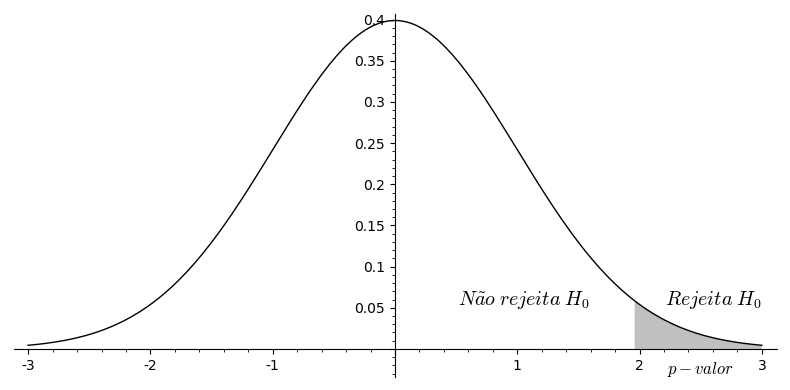
\includegraphics[height=4.75cm]{Unilateral.png}
    \caption{Valor p unilateral da normal}
    \label{fig:unilateral}
\end{figure}
\textbf{Fonte}: Felipe Mendonça, modificado por Augusto César.
\end{frame}

%%%%%%%%%%%%%%%%%% SLIDE 18 %%%%%%%%%%%%%%%%%%%%
\begin{frame}[c]\transfade<1>[duration=0.3] 
\frametitle{P-valor} 
\framesubtitle{Condicionamento}
\begin{itemize}
    \justifying
    \item Outro método para definir um valor p válido, uma alternativa à utilização de (2), envolve condicionar sobre uma estatística suficiente.
    \item Para cada ponto amostral \textbf{x} definimos:
\begin{align}
    p(\textbf{x})=P(W(\textbf{X}) \geq W(\textbf{x})|S=S(\textbf{X}))
\end{align}
\end{itemize}
\end{frame}

%%%%%%%%%%%%%%%%%% SLIDE 18 %%%%%%%%%%%%%%%%%%%%
\begin{frame}[c]\transfade<1>[duration=0.3] 
\frametitle{P-valor} 
\framesubtitle{Condicionamento}
\begin{itemize}
    \justifying
    \item Argumentando como no teorema anterior, mas considerando somente a distribuição única, que é a distribuição condicional de \textbf{X} considerando que $S=s$, vemos que, para qualquer, $0 \leq \alpha \leq 1$, 
\begin{align}
    P(p(\textbf{X}) \leq \alpha| S=s) \leq \alpha
\end{align}
Também, é um p-valor válido.
\end{itemize}
\end{frame}

%%%%%%%%%%%%%%%%%% SLIDE 17 %%%%%%%%%%%%%%%%%%%%
\begin{frame}[c]\transfade<1>[duration=0.3]
\frametitle{P-valor} 
\framesubtitle{Exemplos}
\begin{exampleblock}{\textbf{Exemplo 3} - Teste Exato de Fisher} %Bloco
\begin{itemize}
    \item Sejam $S_{1}$ e $S_{2}$ observações independentes, com $S_{1} \sim Binomial(n_1,p_1)$ e $S_{2} \sim Binomial(n_2,p_2)$. Considere testar $H_0: p_1=p_2$ versus $H_1: p_1 > p_2$.
    \item Seja $S=S_1+S_2$ uma estatística suficiente para $H_0$.
    \item A distribuição condicional $S_1$ dado $S=s$ é hipergeométrica$(n_1+n_2,n_1,s)$, vejamos:
\end{itemize}
\end{exampleblock}
\end{frame}

%%%%%%%%%%%%%%%%%% SLIDE 18 %%%%%%%%%%%%%%%%%%%%
\begin{frame}[c]\transfade<1>[duration=0.3]
\frametitle{P-valor} 
\framesubtitle{Exemplos}
\begin{exampleblock}{\textbf{Exemplo 3} - Teste Exato de Fisher} %Bloco
\begin{itemize}
    \item Sabendo-se que, por definição, a distribuição condicional pode ser reescrita em notação de função de probabilidade da seguinte forma:
    \begin{equation*}
        P_{x|y}(x|y)=\frac{P_{x,y}(x,y)}{P_{y}(y)}
    \end{equation*}
    \item E, se $X,Y$ são independentes, então $P_{x,y}(x,y)=P_{x}(x)\cdot P_{y}(y)$. Sendo assim, temos:
\end{itemize}
\end{exampleblock}
\end{frame}

%%%%%%%%%%%%%%%%%% SLIDE 19 %%%%%%%%%%%%%%%%%%%%
\begin{frame}[c]\transfade<1>[duration=0.3]
\frametitle{P-valor} 
\framesubtitle{Exemplos}
\begin{exampleblock}{\textbf{Exemplo 3} - Teste Exato de Fisher} %Bloco
\begin{align}
    P(S_1=s_1|S_1+S_2=s)&=\frac{P(S_1=s_1,S_1+S_2=s)}{P(S_1+S_2=s)}\nonumber\\
              &=\frac{P(S_1=s_1,S_2=s-S_1)}{P(S_1+S_2=s)}\nonumber\\ 
              &=\frac{P(S_1=s_1,S_2=s-s_1)}{P(S_1+S_2=s)} \nonumber \\
              &=\frac{P(S_1=s_1)P(S_2=s-s_1)}{P(S_1+S_2=s)}
\end{align}
\end{exampleblock}
\end{frame}

%%%%%%%%%%%%%%%%%% SLIDE 19 %%%%%%%%%%%%%%%%%%%%
\begin{frame}[c]\transfade<1>[duration=0.3]
\frametitle{P-valor} 
\framesubtitle{Exemplos}
\begin{exampleblock}{\textbf{Exemplo 3} - Teste Exato de Fisher} %Bloco
Onde, 
    \begin{itemize}
        \item $S_1 \sim Binomial(n_1,s_1)=\binom{n_1}{s_1}p^{s_1}(1-p)^{n_1-s_1}$ 
        \item $S_2 \sim Binomial(n_2,s-s_1)=\binom{n_2}{s-s_1}p^{s-s_1}(1-p)^{n_2-(s-s_1)}$
        \item $S_1 + S_2 \sim Binomial(n1+n2,s)=\binom{n_1+n_2}{s}p^{s}(1-p)^{n_1+n_2-s}$
    \end{itemize}
\end{exampleblock}
\end{frame}

%%%%%%%%%%%%%%%%%% SLIDE 20 %%%%%%%%%%%%%%%%%%%%
\begin{frame}[c]\transfade<1>[duration=0.3]
\frametitle{P-valor} 
\framesubtitle{Exemplos}
\begin{exampleblock}{\textbf{Exemplo 3} - Teste Exato de Fisher} %Bloco
Retomando a equação (9), temos:
 \begin{align*}
    P(S_1=s_1|S_1+S_2=s)
    &=\frac{\binom{n_1}{s_1}p^{s_1}(1-p)^{n_1-s_1}\cdot\binom{n_2}{s-s_1}p^{s-s_1}(1-p)^{n_2-s+s_1}}{\binom{n_1+n_2}{s}p^{s}(1-p)^{n_1+n_2-s}}\\
    &=\frac{\binom{n_1}{s_1}\binom{n_2}{s-s_1}p^{s_1+s-s_1}(1-p)^{n_1-s_1+n_2-s_1+s_1}}{\binom{n_1+n_2}{s}p^{s}(1-p)^{n_1+n_2-s}}\\
    &=\frac{\binom{n_1}{s_1}\binom{n_2}{s-s_1}p^{s}(1-p)^{n_1+n_2-s}}{\binom{n_1+n_2}{s}p^{s}(1-p)^{n_1+n_2-s}}\\
    &=\frac{\binom{n_1}{s_1}\binom{n_2}{s-s_1}}{\binom{n_1+n_2}{s}}=\textit{hipergeométrica}(n1+n2,s)
\end{align*}
\end{exampleblock}
\end{frame}

%%%%%%%%%%%%%%%%%% SLIDE 21 %%%%%%%%%%%%%%%%%%%%
\begin{frame}[c]\transfade<1>[duration=0.3]
\frametitle{P-valor} 
\framesubtitle{Exemplos}
\begin{exampleblock}{\textbf{Exemplo 3} - Teste Exato de Fisher} %Bloco
\begin{itemize}
    \item  O teste definido por este valor p é chamado de Teste Exato de Fisher. 
\end{itemize}
\end{exampleblock}
\end{frame}